\documentclass{standalone}
\usepackage{graphicx}	
\usepackage{amssymb, amsmath, amsthm}
\usepackage{color}

\usepackage{tikz}
\usetikzlibrary{intersections, backgrounds, fadings}

\definecolor{light}{RGB}{220, 188, 188}
\definecolor{mid}{RGB}{185, 124, 124}
\definecolor{dark}{RGB}{143, 39, 39}
\definecolor{highlight}{RGB}{180, 31, 180}
\definecolor{gray10}{gray}{0.1}
\definecolor{gray20}{gray}{0.2}
\definecolor{gray30}{gray}{0.3}
\definecolor{gray40}{gray}{0.4}
\definecolor{gray60}{gray}{0.6}
\definecolor{gray70}{gray}{0.7}
\definecolor{gray80}{gray}{0.8}
\definecolor{gray90}{gray}{0.9}
\definecolor{gray60}{gray}{0.95}

\begin{document}

\begin{tikzpicture}[scale=0.3]
  \pgfmathsetmacro{\dx}{0}
  
  \draw[white] (-19 + \dx, -13) rectangle (19 + \dx, 11);

  \begin{scope}
    \clip (-13 + \dx, -8) rectangle (13 + \dx, 8);
    \node at (0 + \dx, 0) {\includegraphics[width=7.8cm]{gp_scaled.eps}};
  \end{scope}
  
  \draw [->, >=stealth, line width=1] (-13 + \dx, -8) -- +(26, 0);
  \draw [->, >=stealth, line width=1] (-13 + \dx, -8.058) -- +(0, 16);
  
  \node[] at (-6.75 + \dx, -9) { $-1$ };
  \node[] at (0 + \dx, -9) { $0$ };
  \node[] at (6.25 + \dx, -9) { $+1$ };
  \node[] at (0 + \dx, -11.5) { $\displaystyle \frac{x}{\rho}$ };

  \node[] at (-14.5 + \dx, 2.4) { $+1$ };
  \node[] at (-14.5 + \dx, 0) { $\quad0$ };
  \node[] at (-14.5 + \dx, -2.4) { $-1$ };  
  \node[] at (-17.5 + \dx, 0) { $\displaystyle \frac{f(x)}{\alpha}$ };
 
  \pgfmathsetmacro{\dx}{40}
  
  \draw[white] (-21 + \dx, -13) rectangle (17 + \dx, 11);

  \draw[domain=-13:13, smooth, samples=150, line width=1, variable=\x, color=dark] 
    plot ({\x + \dx},{13 * exp(- (\x + 13) * (\x + 13) / 49) - 8});

  \draw[dashed, color=mid, line width=1] (-13 + \dx, 5) -- (13 + \dx, 5);
  \node[text=mid] at (-14.5 + \dx, 5) { $1$ };
  
  \draw[dashed, color=mid, line width=1] (-13 + \dx, -3.1) -- (-6 + \dx, -3.1);
  \draw[dashed, color=mid, line width=1] (-6 + \dx, -8) -- (-6 + \dx, -3.1);
  \node[text=mid] at (-6 + \dx, -9) { $1$ };
  \node[text=mid] at (-14.5 + \dx, -3.1) { $\displaystyle \frac{1}{ e }$ };
  
  \draw [->, >=stealth, line width=1] (-13 + \dx, -8) -- +(26, 0);
  \draw [->, >=stealth, line width=1] (-13 + \dx, -8.058) -- +(0, 16);
  \node[] at (0 + \dx, -11.5) { $\displaystyle \frac{\Delta x}{\rho}$ };
  \node[text=black] at (-18.5 + \dx, 0) { $\displaystyle \frac{k(\Delta x)}{\alpha^{2}}$ };
 
\end{tikzpicture}

\end{document}  